\section{Introduction}
There are infinitely many ways to deform a planar sheet without stretching or tearing it. One can either bend it, form sharp creases by folding it, or combine the two. Folding and bending isometries are different by nature, and historically there has been a dichotomy in the study of the two; Smooth bending deformations are typically studied in differential geometry \cite{do_carmo}, whereas straight folds are often explored in the field of computational origami \cite{origami_book}. Curved folded surfaces \cite{huffman} result as a combination of the two, since folding an inextensible sheet along a curve necessitates global bending around the crease. The elegance of these shapes have garnered the attention of architectures, artists, and industrial designers \cite{arch_geom,tachi2013composite,tachi2011one,buri2011curved,robofold,curved_review}.

Designing curved folded surfaces is a manual and time consuming process, often done using an empirical trial and error approach due to how little theory is known \cite{curved_review,huffmann_reconstructing}. Contrary to classical origami, bending and folding instructions are hard to write down and the fact that multiple creases must be folded simultaneously further complicates the process \cite{StringActuated:2017}. Artists often pre-crease the paper using a ball burnisher or a CNC plotter before carefully folding and bending, making the process of exploration even slower. 

Although manual and slow, playing with paper is currently the only way to fully explore curved folds. Existing works on modeling these surfaces are either limited to previously discovered surfaces \cite{curved_folding_kilian,StringActuated:2017} or model a small partial set of folded surfaces generated by reflections or rotational sweeps \cite{Mitani_ref,mitani2009design}. Modeling the folding process of novel forms remains a challenge \cite{curved_review}. 

\begin{figure*} [h]
	\centering
	\includegraphics[width=\linewidth]{figures/fold_bias_compare}
	\caption{Comparison of the same deformation objective with and without our folding algorithm. Up: Crease patterns given as input (\MiR{have all of them flat}). Center: Applying a deformation objective of the crease patterns without our folding algorithm results in most crease curves being ignored, i.e. not folded. At this stage, one cannot bend these creases without first flattening the surfaes. Down: Result of applying the same deformation with our folding algorithm. Our folding algorithm simultaneously fold all crease points while deforming a surface by adding a bias that effectively push flat points towards a folded configuration while not affecting already folded points. The crease Mountain/Valley assignments, which in these examples are in fact fixed given one choice, are determined automatically without further input. The objective of all of these deformations was a  \textit{curve-constraining flow} \cite{rabi2018shape}, using positional constraints on a single or a part of a crease curve on the surfaces.}
	\label{fig:folded_and_not_folded}
\end{figure*}

In this paper we set out to develop the basic tools for freeform modeling of curved folds, with the objective of aiding the exploration, analysis and study of new curved folded surfaces. Our work builds upon Discrete Orthogonal Geodesic Nets (DOGs) \cite{rabi18,rabi2018shape} as a discrete model for smooth developable surfaces. DOGs are regular quadrilateral meshes with equal angles around each vertex, and unlike other computational models for developables do not suffer from locking of various deformation modes \cite{locking1,locking2,grin_shells}, are not fixed to predetermined rulings directions \cite{pottmann_new,curved_folding_kilian} (see \figref{fig:rulings_problem_curve}) or require remeshing while deforming the surface \cite{StringActuated:2017,SchreckEG2017,Narain}. Given an input crease pattern, we represent a curved folded model as a collection of DOGs, with boundary constraints enforcing equal discrete geodesic curvature along their intersections, as done in \cite{rabi2018shape}.

\begin{figure} [h]
	\centering
	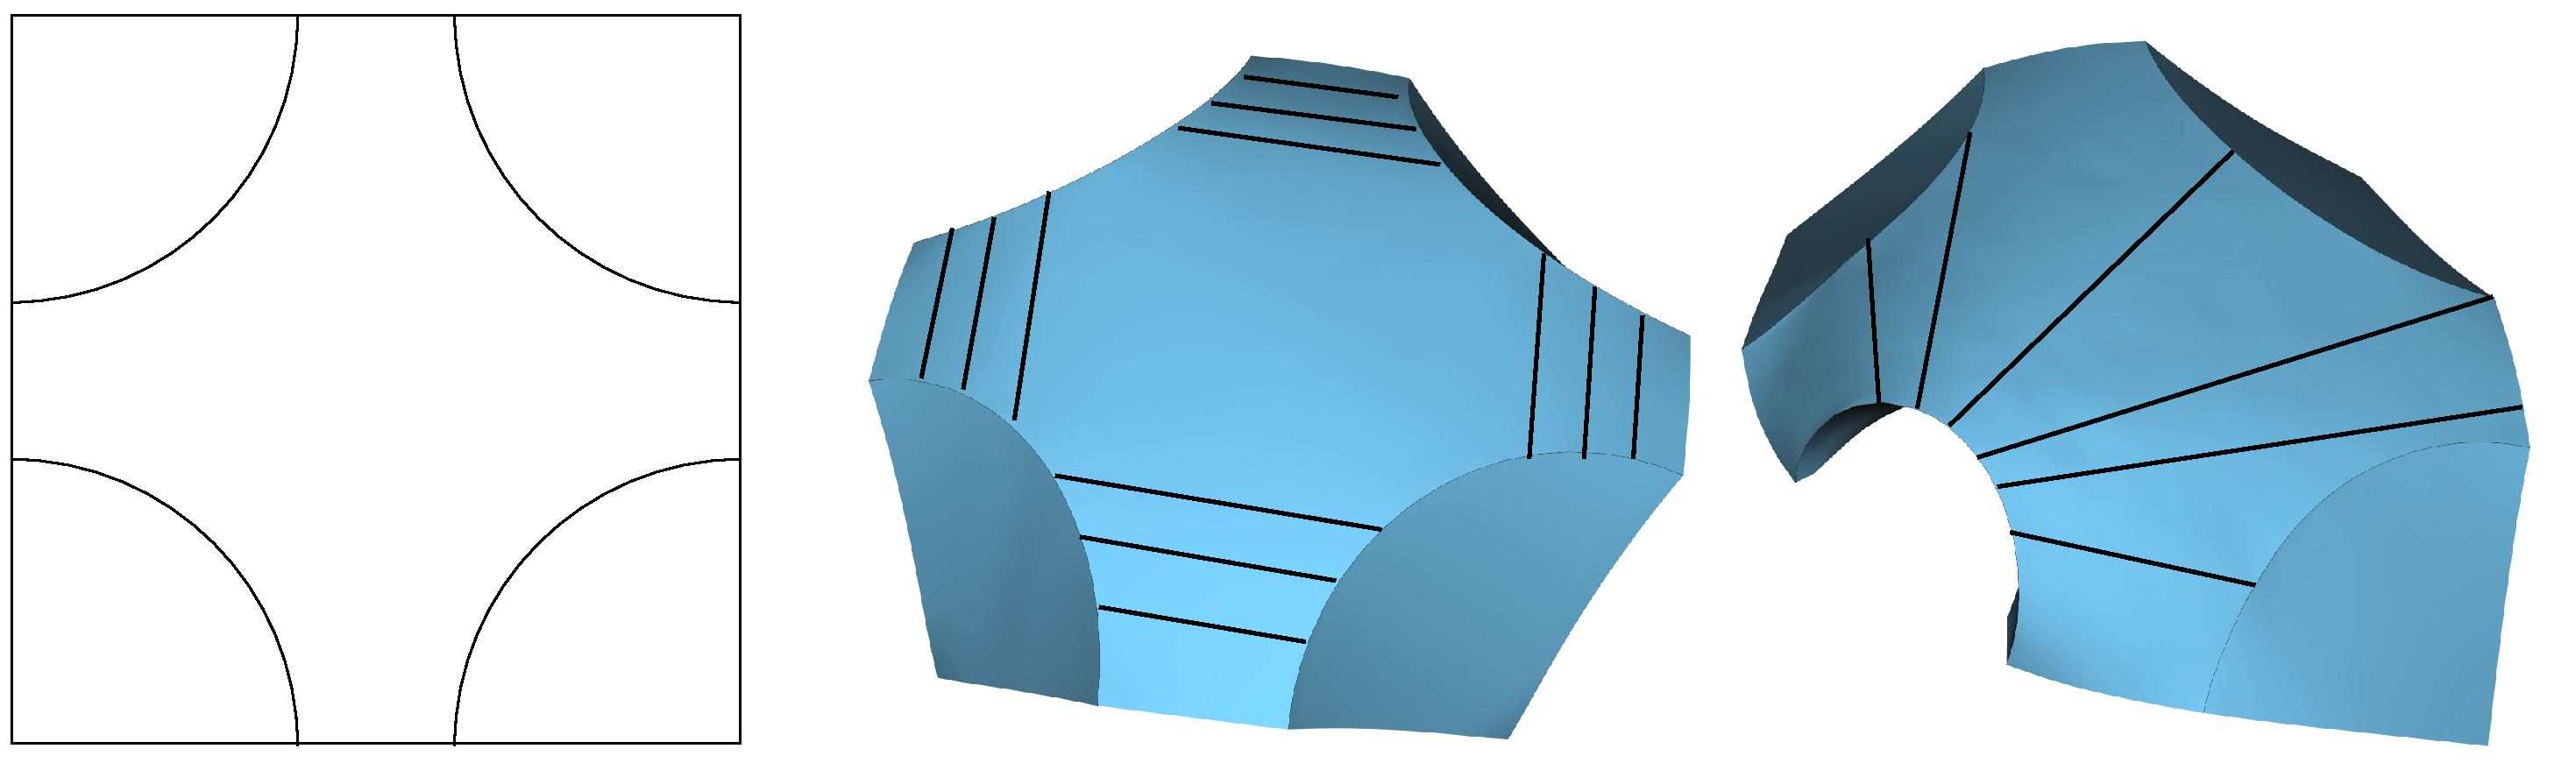
\includegraphics[width=\linewidth]{figures/rulings_problem_curve}
	\caption{Folding and bending of the same curved crease pattern (left) into two different surfaces with some of their ruling lines plotted. Methods that model the ruling directly need to remesh in order to be able to model these surfaces as the rulings can change drastically, connecting vertices at different patches to one another. Representing the curved folded as a piecewise DOG avoid the need in remeshing as a DOG is parameterized by intrinsics invariants: orthogonal geodesics, and does not explicitly encode the developable rulings in its mesh. }
	\label{fig:rulings_problem_curve}
\end{figure}

In practice, deforming a piecewise DOG while keeping the geodesic boundary constraints does not usually results in a model that is folded along all creases (see \figref{fig:folded_and_not_folded}). Our primary goal is to study deformations that bend as well as fold along all creases of a piecewise DOG. Part of the difficulty of modeling these deformations stems from the need to fold all curves simultaneously starting from a flat configuration. \secref{sec:setup} lays the setup for our work, including the problem definition, deseridata and the discrete model we build upon taken from \cite{rabi18,rabi2018shape}. In \secref{sec:folding} we look at the continuous and combinatorial degrees of freedom of curved foldings, detailing how a flat piecewise smooth developable surface is locally a bifurcation point between folded and unfolded configurations. We discuss how folding along a crease given one side of the surface is a binary choice (see \figref{fig:folding_combinatorics}), give a simple discrete charecterization for this choice by looking at supporting planes along the creases, and derive objectives to control the basic properties of folding: dihedral angles and mountain/valley assignments. In \secref{sec:implementation} we translate these derivations into an optimizatioan algorithm capable of enforcing folds while deforming a piecewise DOG. Finally, in \secref{sec:results} we model various curved folded surfaces.

%Section \secref{ At \secref{sec:app}, we show explore a variety of applications for our tools such as wallpaper curved foldings, folding, and modeling while dynamically changing the creased pattern.